\documentclass[border=15pt, multi, tikz]{standalone}
%\usepackage{blocks}
\usepackage{import}
\subimport{../layers/}{init}
\usetikzlibrary{positioning}
\usetikzlibrary{3d} %for including external image
\usepackage[utf8]{inputenc}
\def\ConvColor{rgb:yellow,5;red,7.5;white,5}
\def\ConvTColor{rgb:yellow,4;red,3;white,1}
\def\gConvTColor{rgb:yellow,8;red,3;white,1;green,4}
\def\eConvTColor{rgb:blue,8;red,3;white,4;green,6}
\def\eeConvTColor{rgb:red,10;blue,1;black,4;yellow,2}
\def\ConvReluColor{rgb:yellow,5;red,5;white,5}
\def\PoolColor{rgb:red,1;black,0.3}
\def\imageColor{rgb:white,10}
\def\bnColor{rgb:blue,5;white,3;green,2}
\def\lrColor{rgb:red,1;blue,1;white,3;black,2}
\def\FcColor{rgb:blue,8;red,2.5;white,5}
\def\FcReluColor{rgb:blue,5;red,5;white,4}
\def\SoftmaxColor{rgb:magenta,5;black,7}
\def\strideColor{rgb:black,5;white,3}
\newcommand{\up}{0.25}
\newcommand{\down}{0.25}
\newcommand{\arrowlength}{4}
\newcommand{\copymidarrow}{\tikz \draw[-Stealth,line width =0.8mm,draw={rgb:blue,4;red,1;green,1;black,3}] (-0.3,0) -- ++(0.3,0);}
\begin{document}
\begin{tikzpicture}
\tikzstyle{connection}=[ultra thick,every node/.style={sloped,allow upside
down},draw=\edgecolor,opacity=0.7]
\tikzstyle{copyconnection}=[ultra thick,every node/.style={sloped,allow upside down},draw={rgb:blue,1;red,10;green,1;black,3},opacity=0.7]

\pic[shift={(0,0,0)}] at (0,0,0){Box={name=canvas_1,fill=\FcColor,height=5,width=0.1,depth=5}};
\node[canvas is zy plane at x=0,shift={(0,0,0)}] (temp) at (canvas_1-east)
{
\includegraphics[width=5cm,height=5cm]{./../images/img_0_0}};

\pic[shift={(1,0,0)}] at (canvas_1-east){Box={name=canvas_2,fill=\FcColor,height=5,width=0.1,depth=5}};
\node[canvas is zy plane at x=0,shift={(0,0,0)}] (temp) at (canvas_2-east)
{
\includegraphics[width=5cm,height=5cm]{./../images/img_0_1}};

\pic[shift={(1,0,0)}] at (canvas_2-east){Box={name=canvas_3,fill=\FcColor,height=5,width=0.1,depth=5}};
\node[canvas is zy plane at x=0,shift={(0,0,0)}] (temp) at (canvas_3-east)
{
\includegraphics[width=5cm,height=5cm]{./../images/img_0_2}};

\pic[shift={(1,0,0)}] at (canvas_3-east){Box={name=canvas_4,fill=\FcColor,height=5,width=0.1,depth=5}};
\node[canvas is zy plane at x=0,shift={(0,0,0)}] (temp) at (canvas_4-east)
{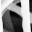
\includegraphics[width=5cm,height=5cm]{./../images/img_0_3}};

\pic[shift={(1,0,0)}] at (canvas_4-east){Box={name=canvas_5,fill=\FcColor,height=5,width=0.1,depth=5}};
\node[canvas is zy plane at x=0,shift={(0,0,0)}] (temp) at (canvas_5-east)
{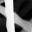
\includegraphics[width=5cm,height=5cm]{./../images/img_0_4}};

%%%%% 

\pic[shift={(3,0,15)}] at (0,0,0){Box={name=canvas_6,fill=\FcColor,height=5,width=0.1,depth=5}};
\node[canvas is zy plane at x=0,shift={(0,0,0)}] (temp) at (canvas_6-east)
{
\includegraphics[width=5cm,height=5cm]{./../images/img_0_5}};

\pic[shift={(1,0,0)}] at (canvas_6-east){Box={name=canvas_7,fill=\FcColor,height=5,width=0.1,depth=5}};
\node[canvas is zy plane at x=0,shift={(0,0,0)}] (temp) at (canvas_7-east)
{
\includegraphics[width=5cm,height=5cm]{./../images/img_0_6}};

\pic[shift={(1,0,0)}] at (canvas_7-east){Box={name=canvas_8,fill=\FcColor,height=5,width=0.1,depth=5}};
\node[canvas is zy plane at x=0,shift={(0,0,0)}] (temp) at (canvas_8-east)
{
\includegraphics[width=5cm,height=5cm]{./../images/img_0_7}};

\pic[shift={(1,0,0)}] at (canvas_8-east){Box={name=canvas_9,fill=\FcColor,height=5,width=0.1,depth=5}};
\node[canvas is zy plane at x=0,shift={(0,0,0)}] (temp) at (canvas_9-east)
{
\includegraphics[width=5cm,height=5cm]{./../images/img_0_8}};

\pic[shift={(1,0,0)}] at (canvas_9-east){Box={name=canvas_10,fill=\FcColor,height=5,width=0.1,depth=5}};
\node[canvas is zy plane at x=0,shift={(0,0,0)}] (temp) at (canvas_10-east)
{
\includegraphics[width=5cm,height=5cm]{./../images/img_0_9}};

%%%%%

\pic[shift={(-3,0,-15)}] at (0,0,0){Box={name=canvas_11,fill=\FcColor,height=5,width=0.1,depth=5}};
\node[canvas is zy plane at x=0,shift={(0,0,0)}] (temp) at (canvas_11-east)
{
\includegraphics[width=5cm,height=5cm]{./../images/img_0_10}};

\pic[shift={(1,0,0)}] at (canvas_11-east){Box={name=canvas_12,fill=\FcColor,height=5,width=0.1,depth=5}};
\node[canvas is zy plane at x=0,shift={(0,0,0)}] (temp) at (canvas_12-east)
{
\includegraphics[width=5cm,height=5cm]{./../images/img_0_11}};

\pic[shift={(1,0,0)}] at (canvas_12-east){Box={name=canvas_13,fill=\FcColor,height=5,width=0.1,depth=5}};
\node[canvas is zy plane at x=0,shift={(0,0,0)}] (temp) at (canvas_13-east)
{
\includegraphics[width=5cm,height=5cm]{./../images/img_0_12}};

\pic[shift={(1,0,0)}] at (canvas_13-east){Box={name=canvas_14,fill=\FcColor,height=5,width=0.1,depth=5}};
\node[canvas is zy plane at x=0,shift={(0,0,0)}] (temp) at (canvas_14-east)
{
\includegraphics[width=5cm,height=5cm]{./../images/img_0_13}};

\pic[shift={(1,0,0)}] at (canvas_14-east){Box={name=canvas_15,fill=\FcColor,height=5,width=0.1,depth=5}};
\node[canvas is zy plane at x=0,shift={(0,0,0)}] (temp) at (canvas_15-east)
{
\includegraphics[width=5cm,height=5cm]{./../images/img_0_14}};


\end{tikzpicture}
\end{document}